\section{State of the art / current knowledge}
\label{sect:star}
\subsection{What results and approaches have already been presented in this or related areas?}
\subsubsection{Berkeley researches replace passwords by measuring brainwaves as a biometric identifier}
\href{http://people.ischool.berkeley.edu/~chuang/pubs/usec13.pdf}
The US Berkeley represents an approach, which turns the brain activity of an user into a biometric identifier. To do this, the Berkeley researchers use a commercial EEG (electroencephalogram), which resembles a Bluetooth headseat with an electrode. This electrode is placed on the users forehead, over the brain's left frontal lobe. The electrode measures the users brainwaves and transmits them via a Bluetooth link to a Device. According to the Berkeley researchers this system has an error rate of below 1 percent.

To ensure that the brain waves of every single person are unique and that they provide enough information to authenticate the user's identity, the Berkley researchers performed tests with participants, which included different kinds of tasks. For example, the participants where asked to just sit and focus on breathing in and out, imagine moving their finger up and down and listen for an audio tone. The participants where also asked to focus on a personalized secret, such as singing a song of their choice. During this tasks, the participants where wearing the EEG which measured their brain waves. As result came out, that not only the measured brainwaves of personalized secrets, but also measured brainwaves of simple tasks, like sitting and focusing on breathing, provided a pattern which makes it possible to authenticate an identity.
\begin{figure}[H]
	\centering
    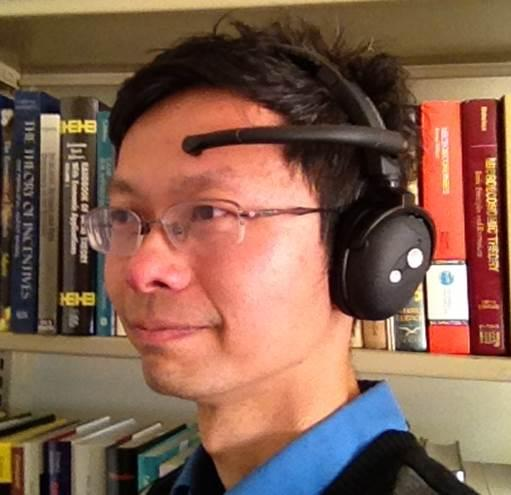
\includegraphics[width=0.5\textwidth]{john_chuang}
    \caption{Professor John Chuang with the Neurosky MindSet brainwave sensor.}
\end{figure}
\subsubsection{Using brain waves as a new biometric feature for authenticating user in real time}
\href{http://www.cscjournals.org/manuscript/Journals/IJBB/volume7/Issue1/IJBB-211.pdf}
Using brain waves as a biometric feature for authenticating was proposed by Kusuma Mohanchandra, Lingaraju G M, Prashanth Kambli \& Vinay in the International Journal of Biometrics and Bioinformat. In this work it has been proved that the brain-wave pattern of every individual is  unique and the signals captured through the  EEG can be used for biometric authentication. This research team used an EEG EPOC headset with 14 channels to measure the brain waves. The collected data, containing the fusion of delta, alpha, theta, beta and gamma brain waves, was merged with the aim to create a way to authenticate the user.

In \cite{kennet} three basic forms of authentication are identified: something-you-have, something-you-know, and something-you-are. According to \cite{kennet}:"
\begin{itemize}
\item Something-you-have can be objects like a key or passport and people have to be very careful not to loose the object or get it stolen.
\item Something-you-know is based on secret knowledge like passwords or PIN codes and the secret must never be written down, forgotten, or told to others.
\item Something-you-are involves person specific features like fingerprints, voice, face, and gait. Authentication based on such features is called biometric authentication. Brain wave based authentication is a combination of something-you-know and something-you-are when the person involved has to think about something specific, but it can also be just something-you-are when the brain waves are used directly as a biometric.
\end{itemize}
 
The most important part of any authentication system is that true identities are verified and that false identities are rejected. In a password system the password is either right or wrong, but with biometric authentication there is an uncertainty involved because the equipment that  measure the biometric feature rarely provide exactly the same data twice. The reason is that external parameters like finger placement, head rotation, facial hair, location etc are present. The challenge is to overcome these problems in such a way that even two slightly different sets of data can be verified to originate from the same person. There is usually a threshold that decide how different
two different sets of data is allowed to be before they are rejected, and as a consequence there is a chance that some clients are falsely rejected and some impostors are falsely verified.
Biometric authentication therefore introduce two error rates: False Non-Match Rate (FNMR), the rate at which clients are falsely rejected by the system, and False Match Rate (FMR), the rate at which impostors are falsely verified by the system. As such the main problem in this thesis is two compare two or more EEG signals and decide whether they are from the same person or not, and get as low FNMR and FMR as possible.''

\subsubsection{Google Glass hack allows brainwave control}
After Google has released his Google Glass, a company called ``This Place``, has developed an app to control the glass over brain waves. However, the app alone is not enough to control the glass with the power of your mind. Normally the Goggle Glass is controlled over voice commands or over a touchpad built into the side of the device. To control the device with brain waves ``This Place`` combined the Google Glass with a Neurosky MindWave headset. The Neurosky MindWave is an EEG-headset to detect brain waves. This is one of the first devices for consumers. Normally this headset will be used to train your brain and it will be delivered with a hand full games. After combining the two devices, the company begined with testing the different kinds of brain waves they could detect. For this reason they created a simple app which implemented a counter starting at 0. When the user concentrated, the app began counting upwards towards 50. When the user started to relax, the counter began returning to 0. After this successfull test, they created an app to show a real-world use, called MindRDR. It allows an user to take a photo and share it over Twitter only by using his mind. Very important to know is that the brain waves only activate the camera app at Google Glass and take a picture. The settings for Twitter were set before. They released their software for free, in hope that other developers can adapt it for other uses.

\subsection{Relation to the international scientific work in the field (international status of the research)}
The very beginning of the existence of brain wave based authentication systems dates back to the 1960's when Vogel discovered a connection between a person's EEG signals and his/her genetic code(DNA). It was proved that every person owns unique brainwaves and it possible to identify a person through his brainwaves. Identical twins where shown to have the same EEG patterns in the same situations and even changes related to aging were similar. 

The brain consists of billions of brain cells called neurons. This neurons have to communicate with each other. For this communication the neurons use electricity called brain waves. This communication is producing a lot of brain waves, which can be detected using sensible sensors such as an EEG. The first person, who confirmed the existence of brain waves and performed the first tests was Hans Berger. There are five different kinds of brain waves and all of them are directly connected to what a person is thinking, doing and feeling:

\begin{itemize}
 \item Gamma (27 Hz and up)
 \item Beta (12 Hz - 27 Hz)
 \item Alpha (8 Hz - 12 Hz)
 \item Theta (3 Hz - 8 Hz)
 \item Delta (0.2 Hz - 3 Hz)
\end{itemize}



This was also explored by \cite{Benedicenti2001} in the year 2001. This researchers used EEG directly as a biometric and their work showed some promising results on this field.


EEG based person authentication was first proposed by \cite{marcel} in “Person authentication using brainwaves (EEG) and maximum a posteriori model adaption”. They proposed the use of  Power Spectral Density as the feature, and a statistical framework based on Gaussian Mixture  Models (GMM) and Maximum A Posteriori Model (MAP) Adaptation on speaker and face  authentication. The potential of their method is shown by simulations using strict train/test protocols and results. 

In \cite{Poulos01personidentification} Poulos, Alexandris and Evangelou performed person identification based on spectral information and presented their results in their work: “On the use of EEG features towards oersin identification via neural networks”. To prove the connection between a person's EEG and genetically specific information, this researchers did experiments with the EEG data of healthy individuals. The proposed method has had a success rate of 80 percent to 100 percent showing that the EEG holds genetic information, which can be used for person identification.


Furthermore, a novel two-stage biometric authentication method was proposed by Palaniappan in \cite{Palaniappan08}. Their results show that the combination of two-stage authentication with EEG features has good potential as a biometric as it is highly resistant to fraud.

\subsection{Description and critical discussion of related scientific work}
The approaches that have been discussed above have succeeded to prove the connection between a person's DNA and her/his brain waves. The approaches clearly show that every single person possesses unique brain waves, which can be used to identify a person. However, a large disadvantage of all of this approaches is that they require the user to wear a big headset with an electrode going across his/her forehead. None of this approaches has succeeded in measuring brain waves from different body parts in order to enable a smaller headset and therefore make it easier for the user to use it in their everyday life.

